\chapter{VAR-Tool}
\label{ch:main-matter}
% \section{Analyse}
% \subsection{As-Is}
% \subsection{To-Be}
\section{UI-Mockup}
  \begin{figure}
    \centering
    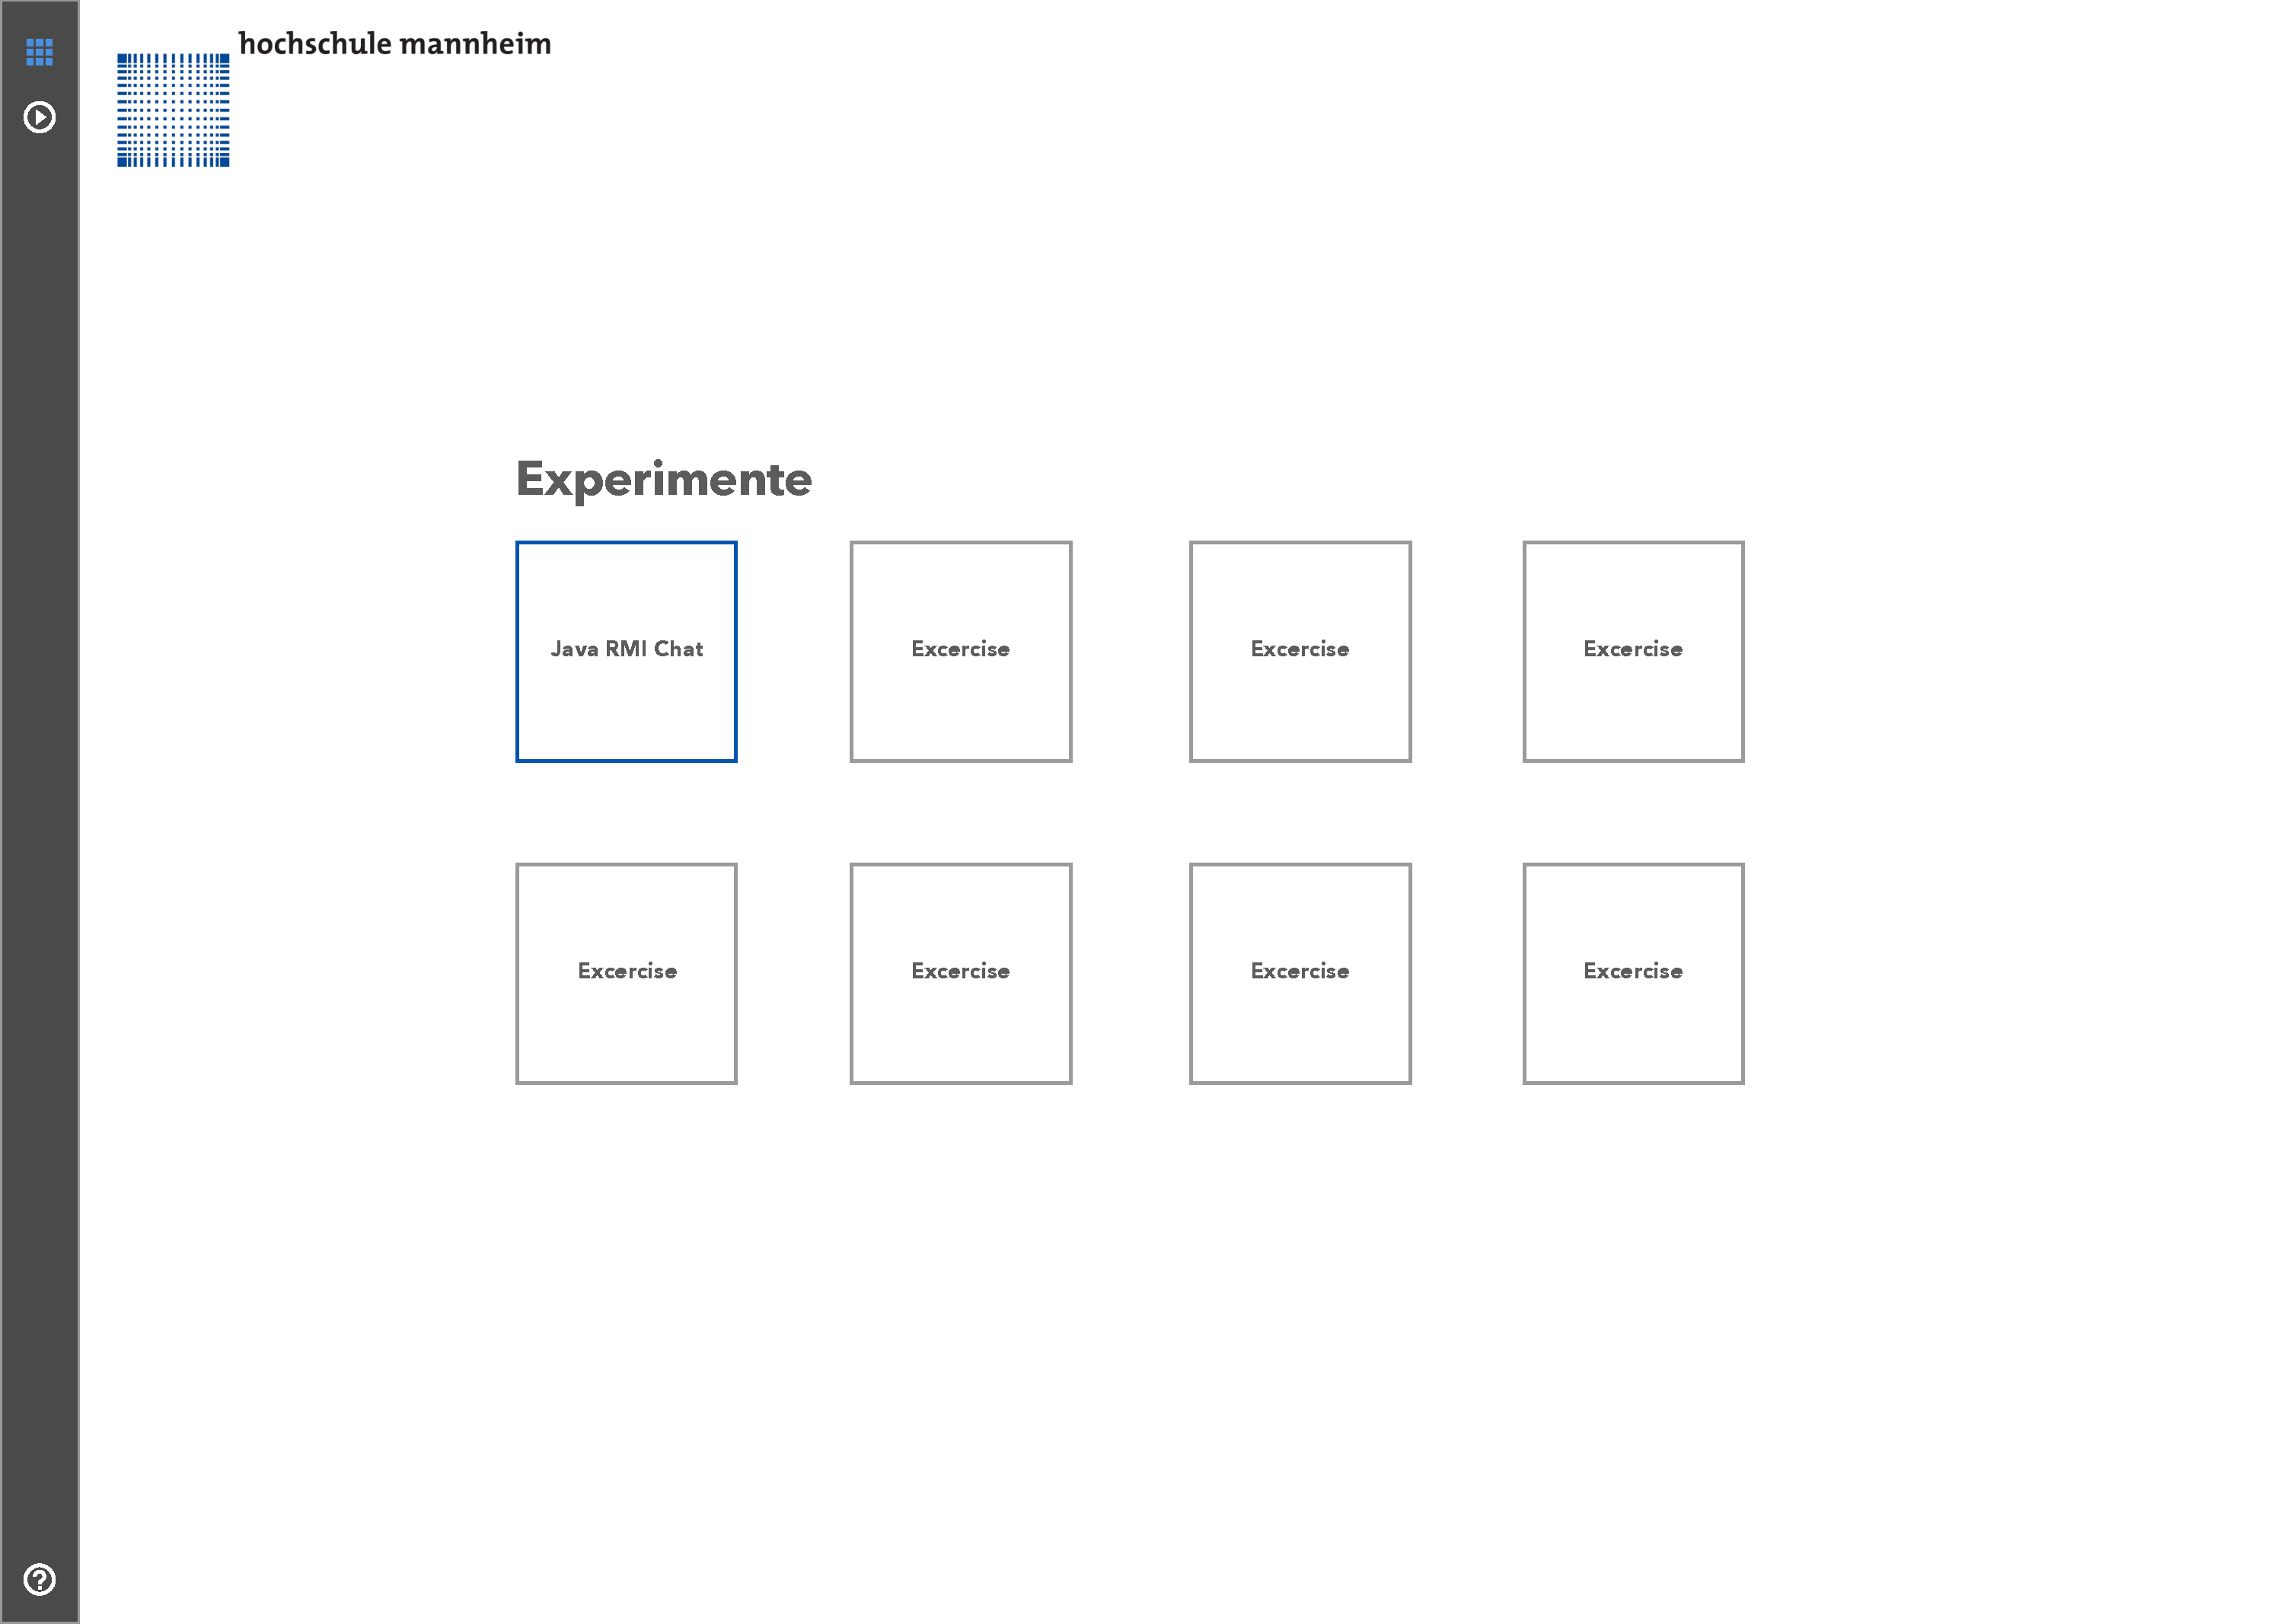
\includegraphics[scale=0.2,page=1]{ui-mockup.pdf}
    \par
    \caption{UI-Mockup: Übersicht der Experimente}
    \label{fig:ui-mockup-1}
  \end{figure}
  \begin{figure}
    \centering
    \includegraphics[scale=0.2,page=2]{ui-mockup.pdf}
    \par
    \caption{UI-Mockup: Experimentenansicht mit verschiedenen Zuständen pro Instanz}
    TODO: improve witdths of mockups
    \label{fig:ui-mockup-2}
  \end{figure}
\section{Architektur}
\subsection{Geschäftsprozesse}
  \begin{figure}
    \centering
    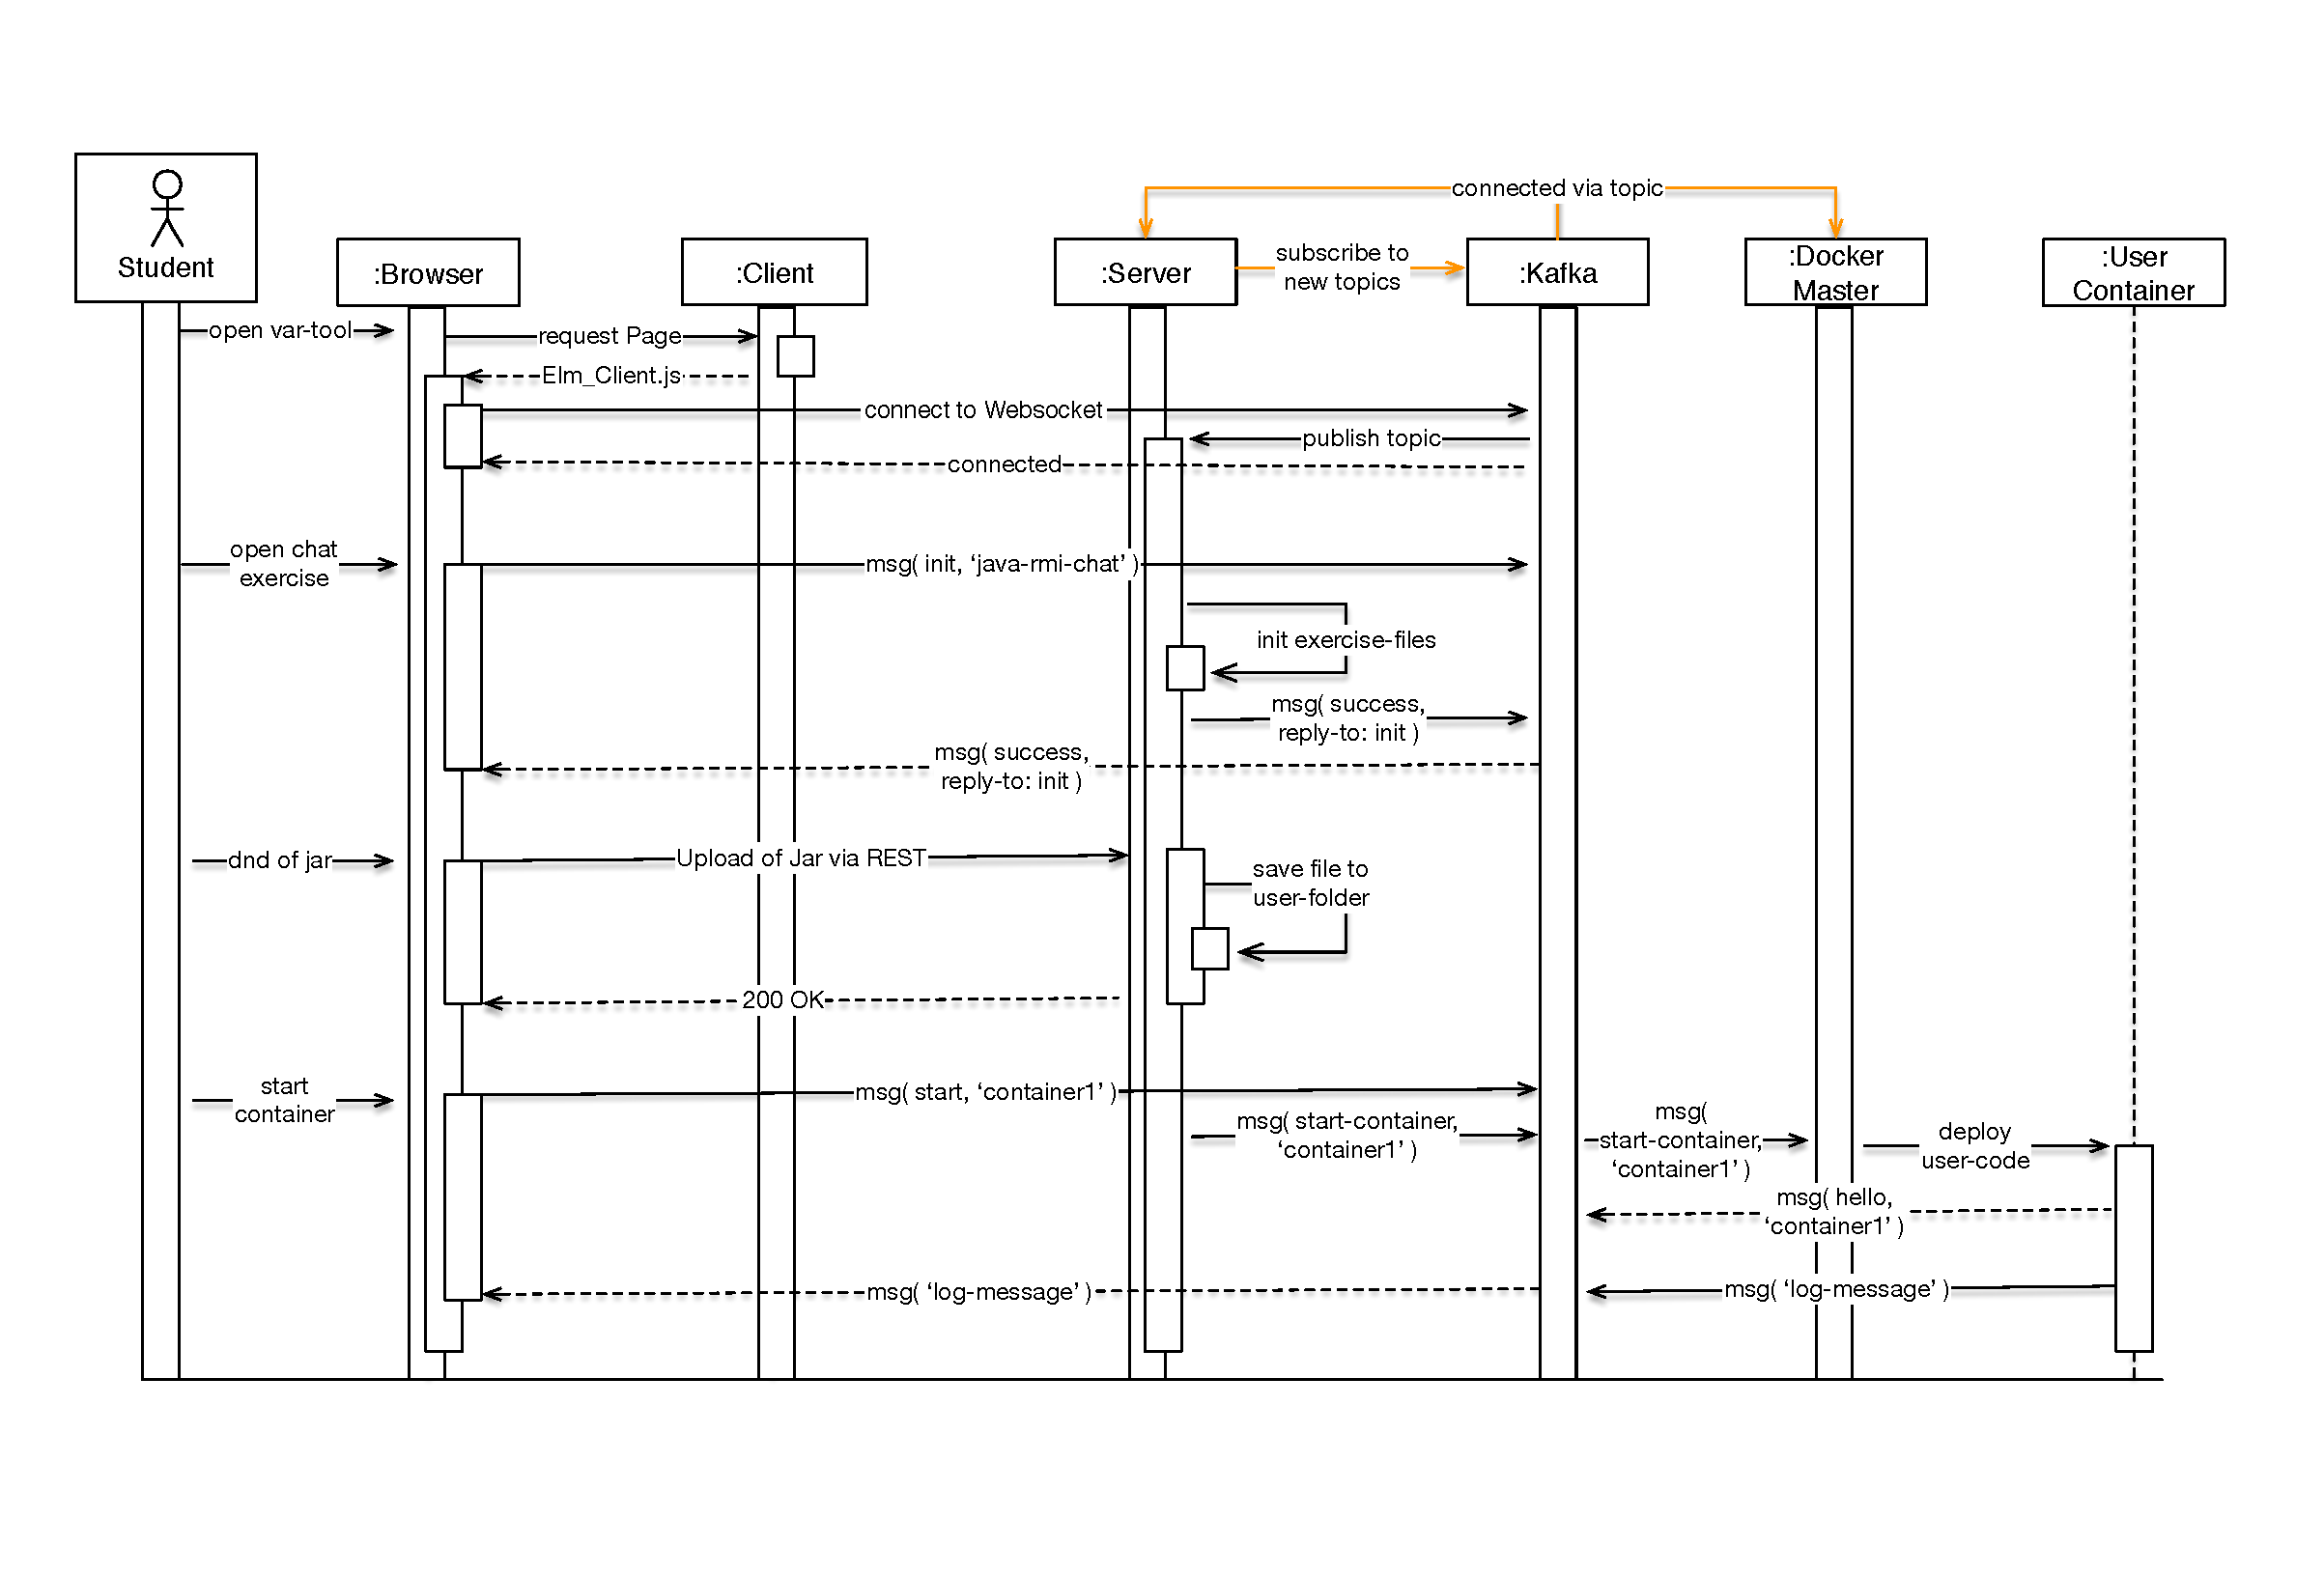
\includegraphics[scale=0.3]{sequence.pdf}
    \par
    \caption{Sequenzdiagramm}
    \label{fig:sequence}
  \end{figure}
\subsection{Netzwerkgrenzen}
  \begin{figure}
    \centering
    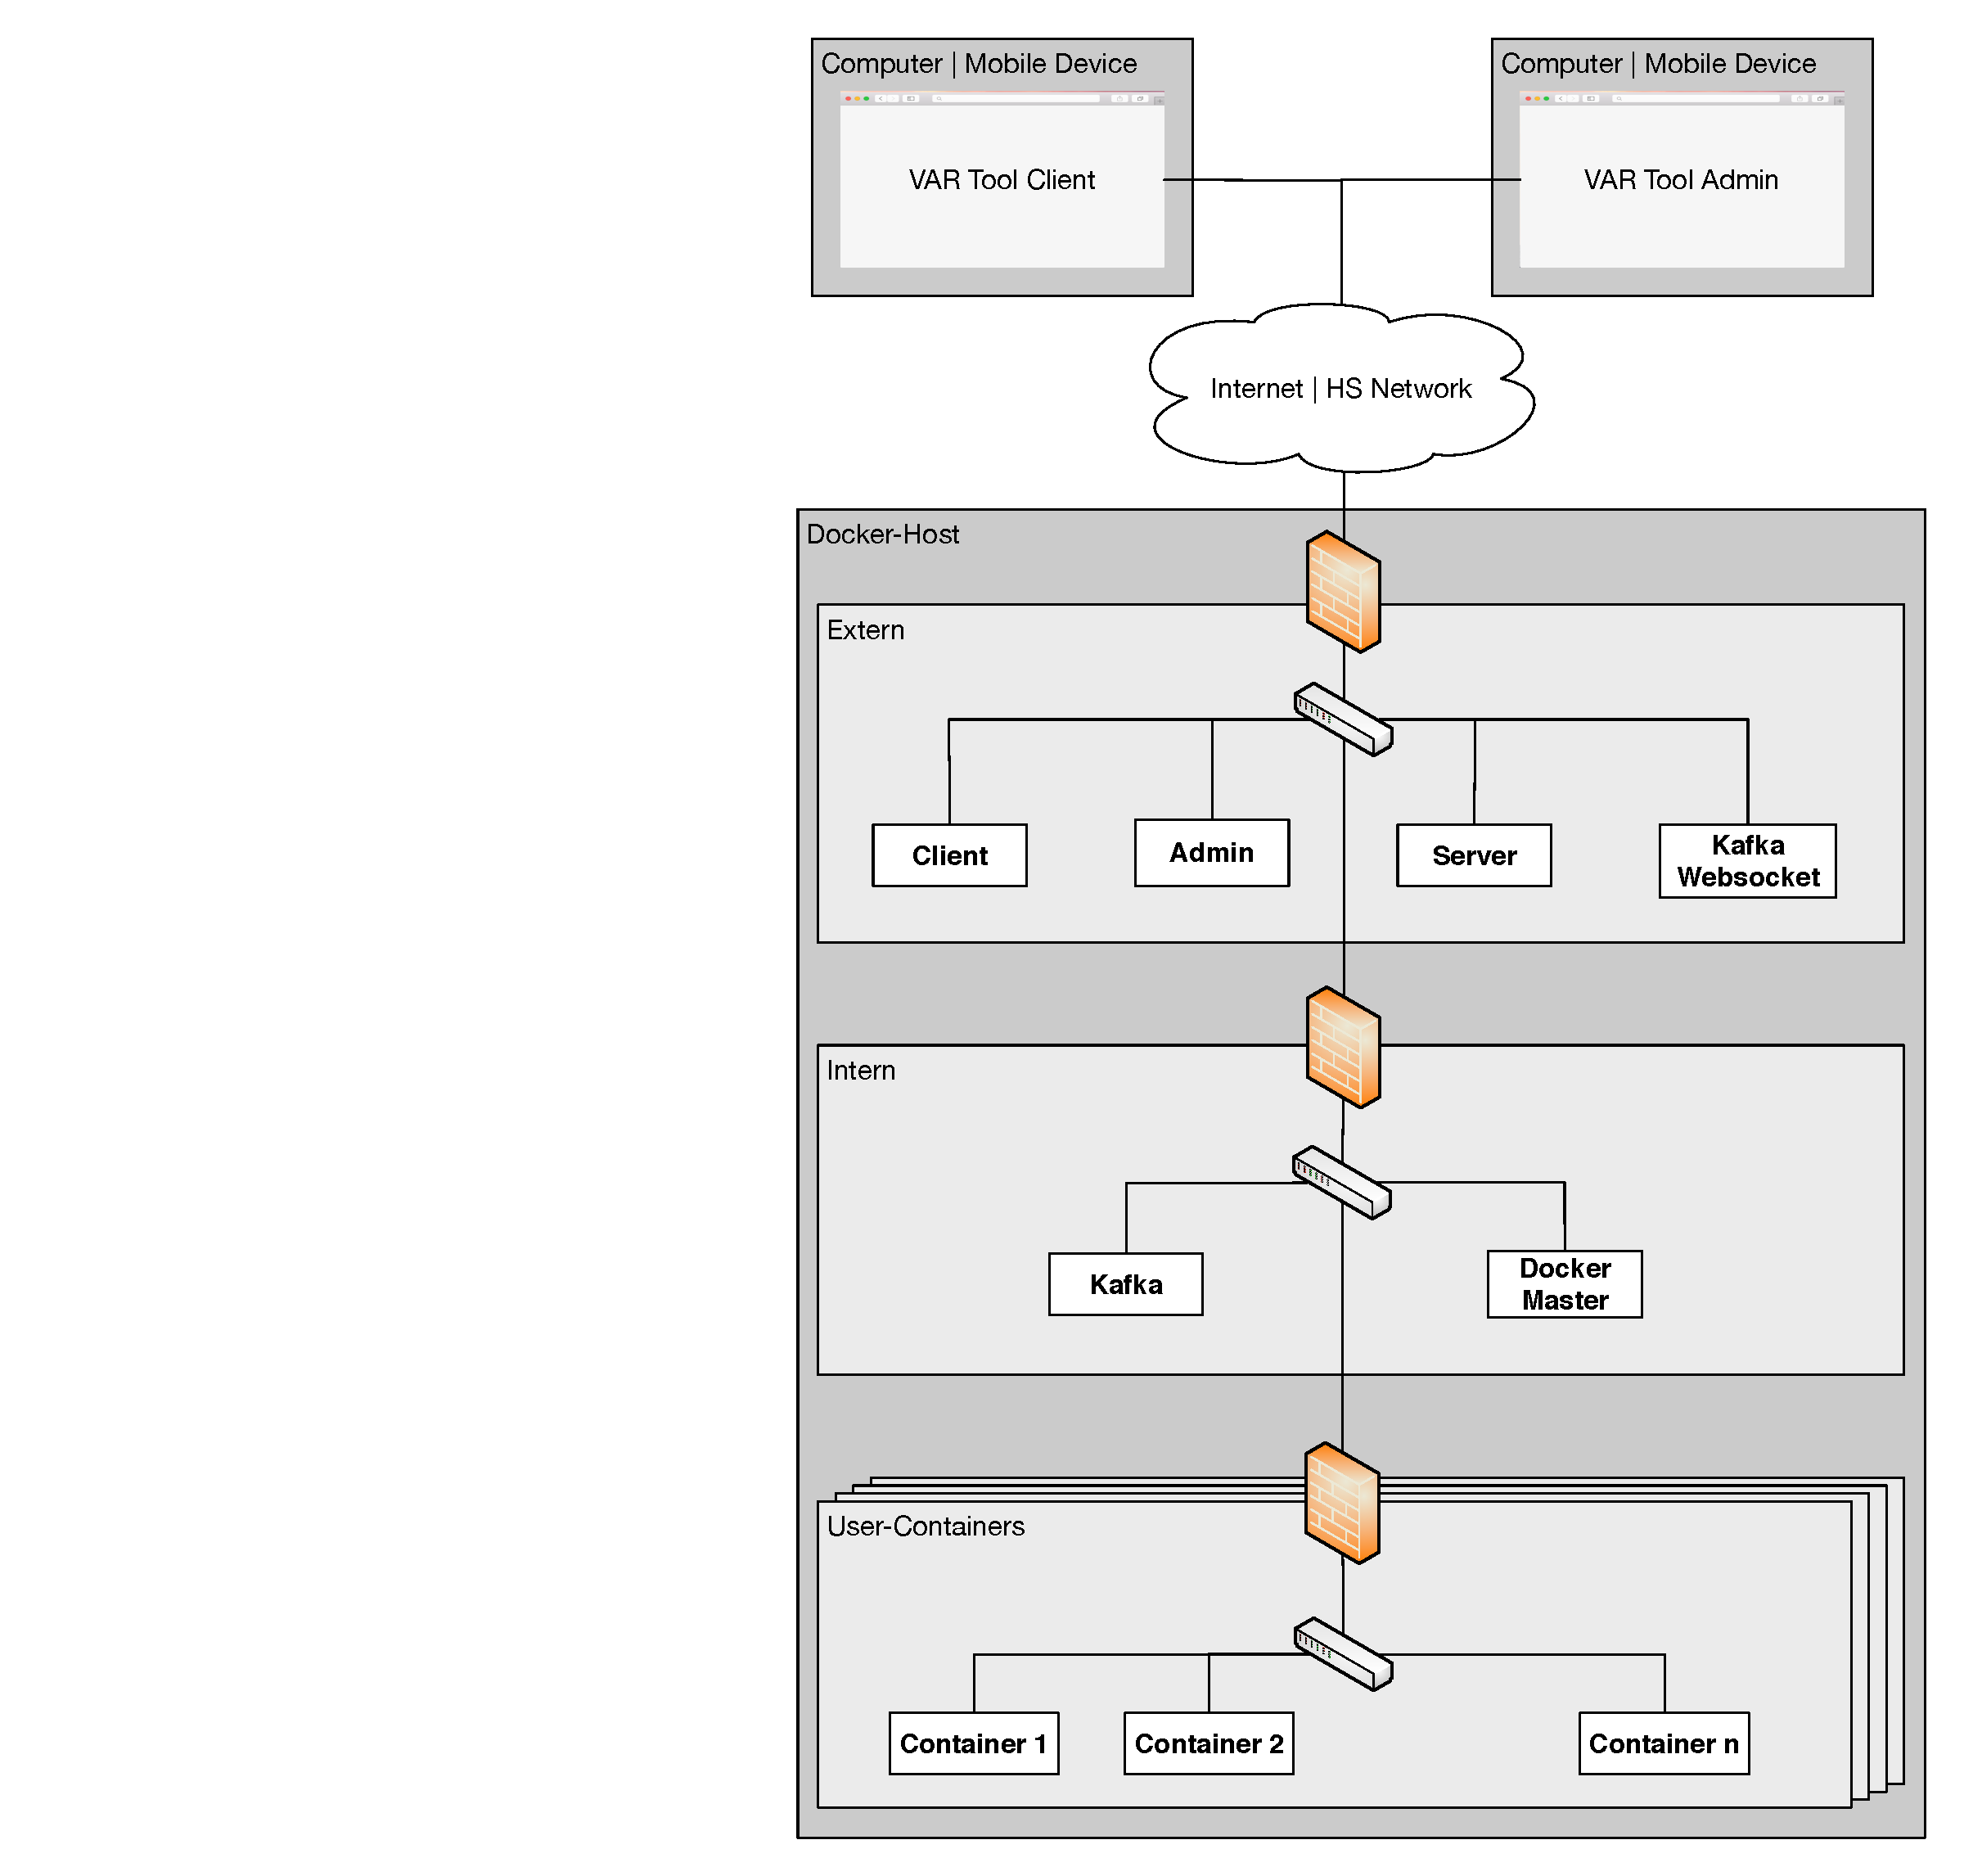
\includegraphics[scale=0.2]{network.pdf}
    \par
    \caption{Netzwerkdiagramm}
    \label{fig:network}
  \end{figure}
\subsection{Deployment}
  \begin{figure}
    \centering
    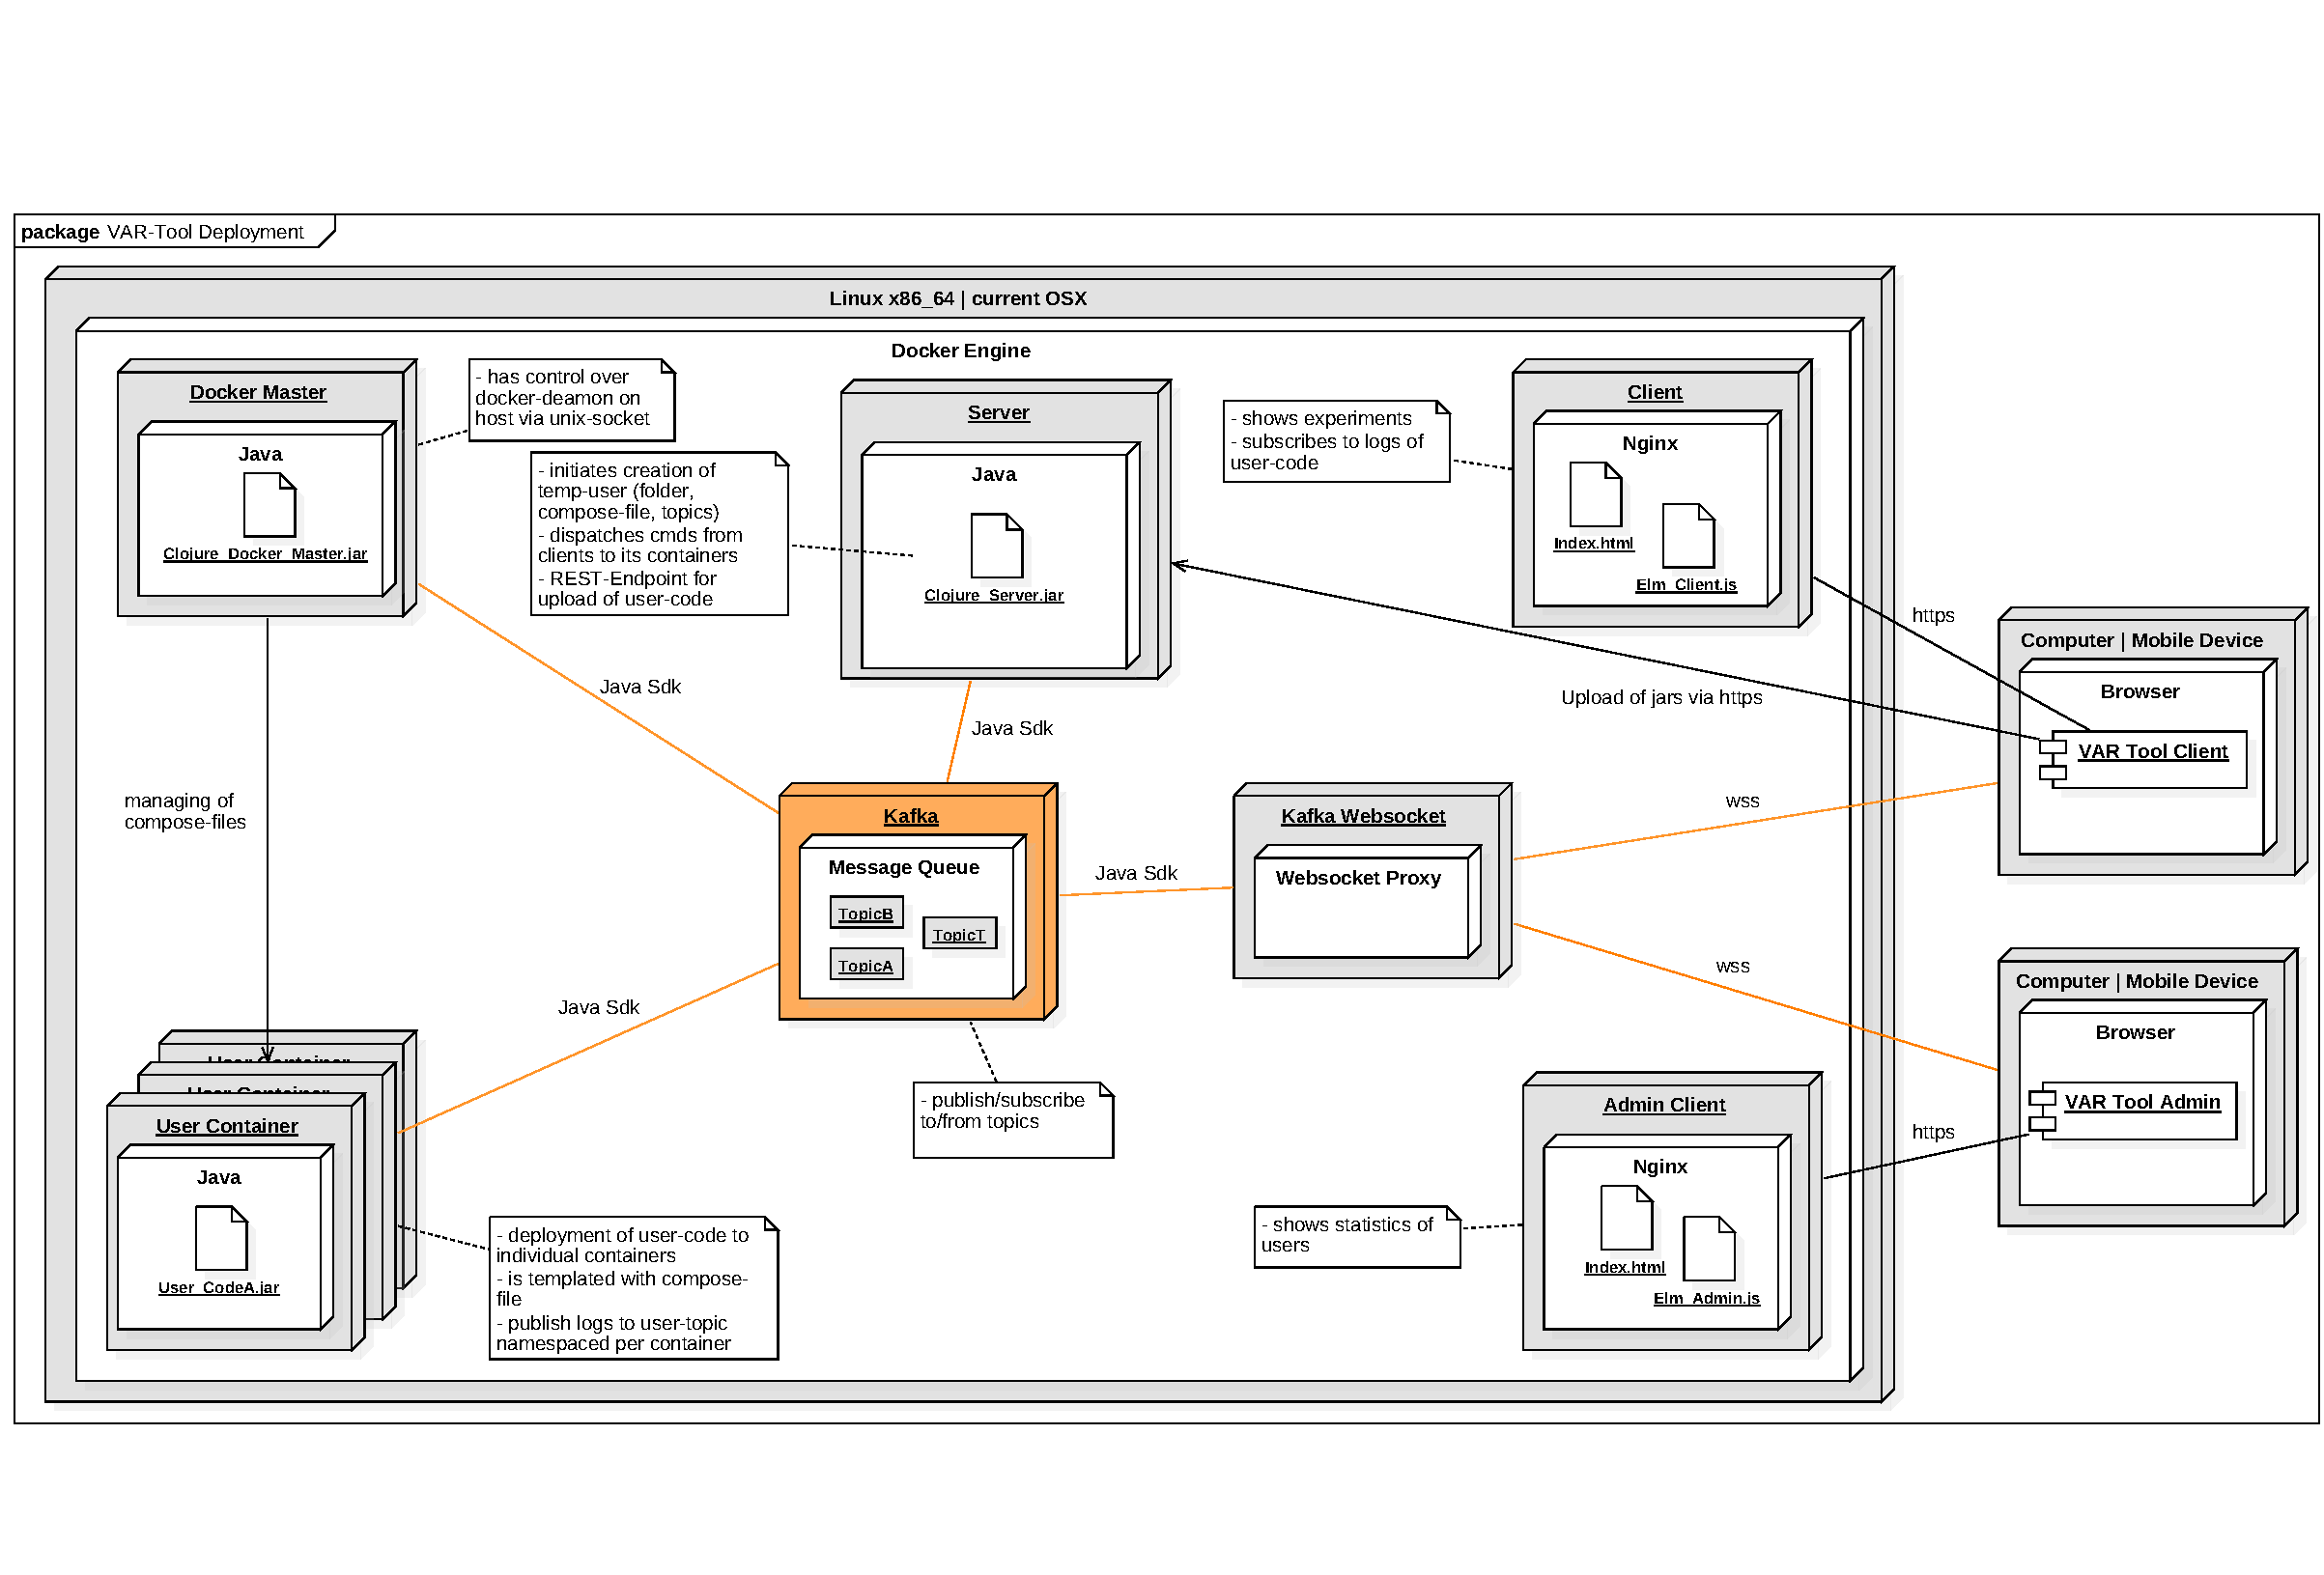
\includegraphics[scale=0.3]{deployment.pdf}
    \par
    \caption{Deploymentdiagramm}
    \label{fig:deployment}
  \end{figure}
\section{Umsetzung}
\subsection{Server}
\subsection{Client}
\section{Installation}
Als erstes wird das Projekt mithilfe von \texttt{git clone \url{https://github.com/jwillem/docker-var.git}} heruntergeladen.
Um die Applikation zu starten, werden zunächst die Installationen von Docker und Docker-Compose benötigt.
Nach einem Ausführen von \texttt{docker-compose build} im Projektverzeichnis kann die App mit \texttt{docker-compose up} gestartet werden.
